\chapter{Battle Mechanics}
\label{chap:battle}
Pokémon GO features two major modes of battle: Nx1 and 3x3\footnote{These are commonly called PvE and PvP
 respectively. I don't like these terms, because Team GO Rocket encounters use the PvP format (despite involving
 a single Trainer), and Gyms use the PvE format (despite involving two Trainers).}.
Nx1 is used for raids, Max Battles, and (in a series of 1x1 matches) assaults on Gyms.
3x3 is used for encounters with Team GO Rocket and Trainer Battles.
All battles work on quanta of 0.5s\footnote{This is a recent change for Raid-style battling.}.
Aside from Trainer Battles, Trainers can make use of items in the screen before
  battle is entered (called the ``lobby'', especially in an Nx1 context), and
  likewise engage Mega evolutions.
Pokémon exchange fast attacks (and, when enough energy has been built up, charged attacks)
  until one side is entirely reduced to zero HP (or surrenders).
Note that attacks typically have different power and energy stats depending on
  whether it's a 3x3 or Nx1 context (\autoref{chap:attacks}).

\section{3x3 battles}
\label{sec:3x3}
Two teams of three Pokémon each are locked in mortal combat.
Each team has one champion fighting at any given time.
The team is ordered: the first Pokémon will emerge first, and should that Pokémon
  faint, the second Pokémon will come in unless the Trainer specifies otherwise.
An active Pokémon can be substituted, but the Trainer cannot perform another
  such substitution for fifty seconds.
There is a four minute (240 second) timer on Trainer Battles, which is not displayed
  until there are twenty seconds remaining or less.
If this timer expires, the Trainer with the most Pokémon remaining wins.
If they have an equal number of Pokémon, the Trainer with less damage to their
  Pokémon (by percentage) wins.

Charged attacks are purchased with energy, fast attacks with time.

\textbf{FIXME}
\textbf{FIXME: mention cmp}


\subsection{Team GO Rocket}
\label{sec:rocket}
\textbf{FIXME}

\section{Nx1 battles}
\label{sec:nx1}
One Pokémon fends off a number of simultaneously attacking Trainers,
  each of whom has one Pokémon active at a time.
There is a timer of 180 seconds for raids below the 5🟉 difficulty level,
  and a timer of 300 seconds for 5🟉 raids.
\textbf{FIXME}

\subsection{Gyms}
\label{sec:gyms}
A team occupies an open gym by leaving a defender there.
All defenders must belong to Trainers from the same team.
Up to six defenders can be left in a gym at once, but only one
  may be left per Trainer.
\textbf{FIXME}

\subsection{Raids}
\label{sec:raids}
A powerful Pokémon, sometimes backed by Team GO Rocket, will seize a gym for an hour.
Assaulting this Pokémon is a raid, or a shadow raid if occupied by a Shadow Pokémon.
Up to twenty Trainers can come together for a raid, with each providing a team of six Pokémon.
If all six are defeated, their Trainer can throw in another team of six.
Only one Pokémon of each Trainer is active at a time, but there is unlimited substitution.
The raid ends when the Pokémon is defeated, no more Pokémon remain fighting,
  or the timer expires.
\textbf{FIXME}

\subsection{Max battles}
\label{sec:maxbattles}
A Dynamax or Gigantamax Pokémon occupies a Power Stop for a period of hours to days.
A team of up to four trainers can fight a Dynamax Battle, each providing up to
  three Dynamax, Gigantamax, or Crowned Pokémon.
A Gigantamax Battle supports up to ten such teams (forty total Trainers, 120 total Pokémon).
Unlike a Raid, new Pokémon cannot be introduced to replace their fallen comrades.
Max Battles introduce a ``Max Meter'', which fills based on damage inflicted and
  energy packs recovered during the battle.
Once it fills, active Pokémon enter their Dynamax or Gigantamax forms, and perform
  up to three Max Moves.
They will not be attacked during this process.
After all three moves, they return to their normal form,
  and the Max Meter returns to zero.
\textbf{FIXME}

\section{Potions and revives}
\begin{figure}[h!]
  \begin{minipage}[t]{0.3\textwidth}
    \begin{center}
    \includegraphics[scale=.4]{images/potion.png}
    \end{center}
    \caption[Potion]{Potion}
    \label{fig:potion}
  \end{minipage}
  \begin{minipage}[t]{0.3\textwidth}
    \begin{center}
    
\includegraphics[scale=.4]{images/superpotion.png}
    \end{center}
    \caption[Super potion]{Super}
    \label{fig:superpotion}
  \end{minipage}
  \begin{minipage}[t]{0.3\textwidth}
    \begin{center}
    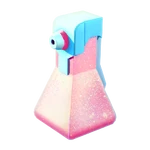
\includegraphics[scale=.4]{images/Hyper_Potion.png}
    \end{center}
    \caption[Hyper potion]{Hyper}
    \label{fig:hyperpotion}
  \end{minipage}
\end{figure}
Damage to your Pokémon persists after a Raid, Max Battle, or 3x3 with Team GO Rocket ends.
Those which fainted will remain fainted until a Revive or Max Revive is applied.
While fainted, they cannot be brought into battle.
Powering up a fainted Pokémon will revive them with minimal HP (\autoref{sec:plevel}),
  while evolving one restores full HP (\autoref{sec:evolution}).
A regular Revive brings the Pokémon back with half of MHP; the Max Revive restores full HP.
If the Pokémon isn't fainted, but merely damaged, four levels of Potion
  restore various amounts of HP, never exceeding MHP\@.
Hyper Potions heal up 200 HP, sufficient to restore all but the bulkiest Pokémon to MHP.
For them, there exist Max Potions, which go all the way to MHP.
Potions cannot be applied to fainted Pokémon; they must first be revived.
Potions and Revives are level-gated, but once unlocked can be semi-randomly acquired
  from Gifts (\autoref{sec:gifts}),
  from advancing to a new Level (\autoref{table:levelitems}),
  from spinning Pokéstops (especially at Gyms, particularly when occupied by your team, and when you have a badge for the gym),
  in the three 7-day streak awards,
  by completing Routes,
  by winning Raids,
  and in the daily free package from the Store.
\begin{table}[ht]
\begin{center}
\begin{tabular}{ll}
Item & Effect \\
\Midrule
Potion & Restore 20 HP, not to exceed MHP\\
Super Potion & Restore 50 HP, not to exceed MHP\\
Hyper Potion & Restore 200 HP, not to exceed MHP\\
Max Potion & Restore to full MHP\\
Revive & Revive with half of MHP\\
Max Revive & Revive with full MHP\\
\end{tabular}
\end{center}
\caption{Potions and revives}
\label{table:potions}
\end{table}
\begin{figure}[h!]
  \begin{minipage}[t]{0.3\textwidth}
    \begin{center}
    
\includegraphics[scale=.4]{images/Max_Potion.png}
    \end{center}
    \caption[Max potion]{Max}
    \label{fig:maxpotion}
  \end{minipage}
  \begin{minipage}[t]{0.3\textwidth}
    \begin{center}
    
\includegraphics[scale=.4]{images/revive.png}
    \end{center}
    \caption[Revive]{Revive}
    \label{fig:revive}
  \end{minipage}
  \begin{minipage}[t]{0.3\textwidth}
    \begin{center}
    
\includegraphics[scale=.4]{images/maxrevive.png}
    \end{center}
    \caption[Max revive]{Max revive}
    \label{fig:maxrevive}
  \end{minipage}
\end{figure}
